\documentclass[11pt, oneside]{article} 
\usepackage{geometry}
\geometry{letterpaper} 
\usepackage{graphicx}
	
\usepackage{amssymb}
\usepackage{amsmath}
\usepackage{parskip}
\usepackage{color}
\usepackage{hyperref}

\graphicspath{{/Users/telliott_admin/Dropbox/Tex/png/}}
% \begin{center} 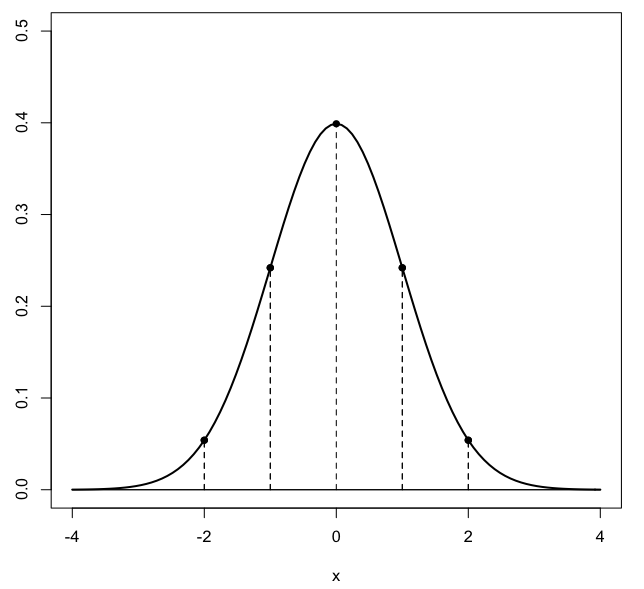
\includegraphics [scale=0.4] {gauss3.png} \end{center}

\title{Infinite series}
\date{}

\begin{document}
\maketitle
\Large
Strang says the most important series of all is the \emph{geometric} series and I think that's right:
\[ 1 + x + x^2 + x^3 + \dots = \sum_{n=0}^{\infty} x^n \]
Probably the most well-known example has $x = 1/2$:
\[ 1 + \frac{1}{2} + \frac{1}{4} + \frac{1}{8} + \dots \]

Although the number of terms in this series is infinite, the sum is finite.  Here is a "visual proof" for the sum starting at the second term:
\begin{center} 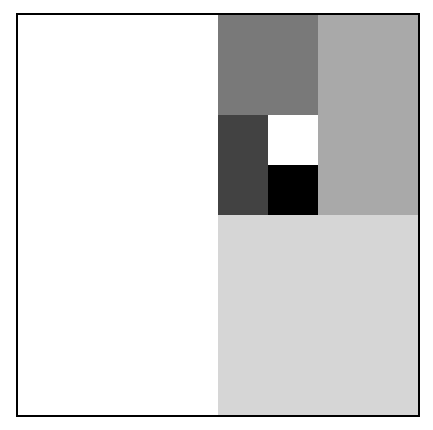
\includegraphics [scale=0.3] {series1.png} \end{center}

In this figure, we see that $1/2 + 1/4 + 1/8 + \dots = 1$.  So the sum of the series written above is equal to $1 + 1 = 2$.

We'd like to determine algebraically or analytically what the sum is. There is a simple approach to this.  Let
\[ S = 1 + x + x^2 + x^3 + \dots \]
\[ Sx =  x + x^2 + x^3 + \dots \]
\[ S - Sx = 1 \]
\[ = S(1-x)  \]
\[ S = \frac{1}{1-x} \]
This seems to work.  For the first example, with $x=1/2$, we obtain $2$, as expected (starting the series at $1$).  Also, multiplying
\[ (1 - x) (1 + x + x^2 + x^3 + \dots) \]
apparently cancels every term after the first $1$.

Unfortunately, there's a problem.  Above, we assumed that $S$ is a number.  But infinity is \emph{not} a number.  For some values of $x$, the series is not finite.  

Consider $x=1$:
\[ 1 + x + x^2 + x^3 + \dots = 1 + 1 + 1 + 1 +  \dots \] 
And when $x = -1$, the series oscillates:
\[ 1 - 1 + 1 - 1 +  \dots \]
So the answer we obtained before is the value of the sum, but only when that value exists.

The careful way to analyze this says, let us look at sums when we stop the series early, after $n$ terms.  The partial sum $S_n$ is
\[ S_n = 1 + x + x^2 + x^3 + \dots + x^n \]
This value, $S_n$ is certain to be finite if $x$ is finite.  We do what we did before.
\[ (1 - x) S_n = S_n - x S_n \]
On the right-hand side, multiplication by $1-x$ produces a "telescoping sum" so that
\[ =  1 + x - x + x^2 - x^2 \dots + x^n - x^n - x^{n+1} \]
\[ = 1 - x^{n+1} \]

Division gives
\[ S_n = \frac{1 - x^{n+1}}{1-x} = \frac{1}{1-x} - \frac{x^{n+1}}{1-x} \]
To evaluate the infinite series, we ask what this limit is as $n$ grows larger
\[  \lim_{n \rightarrow \infty} \frac{x^{n+1}}{1-x} \]
If 
\[ x^{n+1} \rightarrow 0 \ \ \text{as} \ \ n \rightarrow \infty \]
then the series converges.  This only happens when $|x| < 1$ and we call this range of values the "radius of convergence" of the series.
\[    \sum_{n=0}^{\infty} x^n = \frac{1}{1-x} \ \ \iff \ \ \ -1 < x < 1 \]
For something like
\[  \sum_{n=0}^{\infty} ax^n = a + ax + ax^2 + \dots \]
write
\[ \sum_{n=0}^{\infty} ax^n = a \sum_{n=0}^{\infty} x^n = \frac{a}{1-x} \]
To compute the sum of a geometric series, use this formula:  
\[  \frac{\text{first term}}{1 - \text{common ratio}} \]

example
\[  \sum_{n=1}^{\infty} \frac{1}{2^n} \]
This is the classic geometric series.  The common ratio is $1/2$.  Since the ratio is between $-1$ and $1$, the series converges.  The first term is $1/2$ and the value of the sum is:
\[ \frac{1/2}{(1 - 1/2)} = 1 \]

Alternatively
\[  \sum_{n=0}^{\infty} \frac{1}{2^n} \]
This is the same as before except the first term is $1$ and the sum is
\[    \frac{1}{(1 - 1/2)} = 2 \]

\subsection*{Repeating decimals}
Consider
\[  \sum_{n=1}^{\infty} \frac{1}{10^n} \]
\[ = \frac{1}{10} + \frac{1}{100} + \frac{1}{1000} + \dots \]
This one is also a geometric series.  The sum is obviously
\[ = 0.1111 \dots \]
\[ = \frac{1}{9} \]
But the formula works here too.

Other interesting repeating decimals are:
\[ n = 0.012345679012345679012345679 \dots \]
To see this in a more familiar form, multiply by $10^9$
\[ 1,000,000,000 \ n = 12345679.0123456790123456790 \dots \]
The difference is 
\[ 999,999,999 \ n = 12,345,679 \]
\[ \frac{12345679}{999,999,999} = \frac{1}{81} \]

or even
\[ \frac{1}{243} = 0.004115226337448559670781893 \dots \]
The repeat has 25 digits.

\url{http://mathworld.wolfram.com/243.html}

\subsection*{Harmonic series}
The harmonic series is
\[ \sum_{n=1}^{\infty} \frac{1}{n} = \frac{1}{1} + \frac{1}{2} + \frac{1}{3} + \frac{1}{4} + \frac{1}{5} + \dots \]
Obviously, $n$ cannot be equal to $0$ so we start at $n=1$.

The harmonic series diverges.  A classic proof is to group the terms:
\[    = \frac{1}{1} + \frac{1}{2} + (\frac{1}{3} + \frac{1}{4}) + (\frac{1}{5} + \frac{1}{6} + \frac{1}{7} + \frac{1}{8}) + \dots \]
    
Clearly, we can continue this grouping operation forever.  The next group has denominators from $9 \dots 16$, and in general, from $2^{n-1} + 1$ up to $2^n$.
    
The sum for each group is at least $1/2$, so the series is larger term by term than:
\[ = \frac{1}{1} + \frac{1}{2} + \frac{1}{2} + \frac{1}{2} + \frac{1}{2} + \dots \]

But this series is clearly divergent, so the harmonic series, whose sum is larger term by term, also diverges.

According to Acheson, this proof dates to 1350 and can be attributed to the French scholar, Nicole Oresme.

A fun fact about this series is that if we consider the related series of inverse primes, that is
\[ \sum_{n=2}^{\infty} \frac{1}{p} = \frac{1}{2} + \frac{1}{3} + \frac{1}{5} + \frac{1}{7} + \frac{1}{11} + \dots \]
This sum \emph{also} diverges (see Maor's book on infinity).  Maor also says that the $N$th partial sum of the harmonic series, the sum of the first $N$ terms, obeys this inequality:
\[ \ln N < S_N < \ln N + 1 \]

From this, we deduce that the sum of the first one googol ($10^{100}$) terms of the series, is just a bit more than $230$.  Even so, the harmonic series diverges.

Here is another proof:

\begin{center} 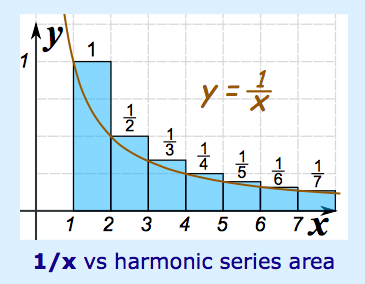
\includegraphics [scale=0.6] {harmonic_integral.png} \end{center}

The area under the boxes is equal to the sum of the harmonic series.  We will show that the integral, the area under the smooth curve, diverges to $\infty$.  Since the harmonic series is larger than that, it also diverges.

The integral is
\[ I = \int_1^{\infty} \frac{1}{x} \ dx \]
which we evaluate by substituting a finite upper limit
\[ I = \int_1^{a} \frac{1}{x} \ dx \]
\[ = \ln x \ \bigg |_1^a = \ln a \]
But as $a \rightarrow \infty$, the logarithm also tends to $\infty$, so it diverges.

\subsection*{Related to geometric series}
Again, the geometric series is:
\[    S = 1 + x + x^2 + x^3 + \dots \]
Differentiate.  The right-hand side is
\[ 1 + 2x + 3x^2 + 4x^3 + \dots \]
and the left-hand side is
\[ \frac{d}{dx} \ [ \ \frac{1}{1-x} \ ] \ = \frac{1}{(1-x)^2} \]

Try multiplying out
\[ (1-x) (1 + 2x + 3x^2 + 4x^3 + \dots ) \]
\[ = 1 + 2x - x + 3x^2 - 2x^2 + 4x^3 - 3x^3 +  \dots ) \]
\[ = 1 + x + x^2 + x^3 + \dots \]
\[ = \frac{1}{1-x} \]

It checks.  And since
\[    (\frac{1}{1-x})(\frac{1}{1-x}) = \frac{1}{(1-x)^2} \]
\[    (1 + x + x^2 + \dots) (1 + x + x^2 + \dots) \]
\[    = 1 + 2x + 3x^2 + 4x^3 + 5x^4 + \dots \]

\subsection*{Integrate}
\[    \frac{1}{1-x} = 1 + x + x^2 + x^3 + \dots \]
\[    \int \frac{1}{1-x} \ dx = \int 1 + x + x^2 + x^3 + \dots \ dx \]
\[     -\ln |1-x| = x + \frac{x^2}{2} + \frac{x^3}{3} + \frac{x^4}{4} + \dots \]

Let $x = 1/2$
\[ - \ln \frac{1}{2} = \ln 2 = \frac{1}{2} + \frac{1}{8} + \frac{1}{24} + \frac{1}{64} + \dots \]
We can calculate $\ln 2$.

This converges fairly slowly.  Still 20 terms gives six places correct ($0.693147$).

\subsection*{Change variables}
Start with the geometric series
\[    1 + x + x^2 + x^3 + \dots \]
Replace $x$ by $-x^2$:
\[    1 - x^2 + x^4 - x^6 + \dots = \frac{1}{1+x^2} \]

Now, does that right-hand side look familiar?  Perhaps not, if you haven't seen the trigonometric functions.  Take it on faith that

\[    \int \frac{1}{1+x^2} \ dx = \tan^{-1} x \]
where $ \tan^{-1}$ or arc tangent is the \emph{inverse function} to the tangent.  That is, if

\[ x = \tan \theta \]
then
\[ \theta = \tan^{-1} x \]

Integrate the left-hand side:
\[    \int 1 - x^2 + x^4 - x^6 + \dots \ dx = x - \frac{x^3}{3} + \frac{x^5}{5} - \frac{x^7}{7} \]

Set $x = 1$.  The angle with $\tan^{-1} \theta = 1$ is $\theta = \pi/4$.  Thus:
\[    \tan^{-1} 1 = \frac{\pi}{4} = 1 - \frac{1}{3} + \frac{1}{5} - \frac{1}{7} \]
We have found a series that equals $\pi$!  How cool is that?

This particular series converges extremely slowly.  It can be improved in a couple ways.  One way is by combining adjacent terms:  $1/5 - 1/7 = 2/35;  1/9 - 1/11 = 2/99$ and so on.

Another way is to set $x = 1/\sqrt{3}$, then the angle with that tangent is $\pi/6$ (recall that $\sin \pi/6 = 1/2$ and $\cos \pi/6 = \sqrt{3}/2$).

So
\[    \frac{\pi}{6} = \frac{1}{\sqrt{3}} - \frac{1}{3} \ (\frac{1}{\sqrt{3}})^3 +  \frac{1}{5} \ (\frac{1}{\sqrt{3}})^5 -  \frac{1}{7} \ (\frac{1}{\sqrt{3}})^7 + \dots \]
\[     = \frac{1}{\sqrt{3}} (1 - \frac{1}{3} \ (\frac{1}{3}) + \frac{1}{5} \ (\frac{1}{3})^2 + \frac{1}{7} \ (\frac{1}{3})^3 \dots) \]
\[    = \frac{1}{\sqrt{3}} (1 - \frac{1}{9} + \frac{1}{45} - \frac{1}{189} + \frac{1}{729} - \frac{1}{2673}) \]

\begin{verbatim}
    >>> from math import sqrt
    >>> r = 1/sqrt(3)
    >>> r * (1 - 1.0/9 + 1.0/45 - 1.0/189 + 1.0/729 - 1.0/2673)
    0.5235514642438139
    >>>
\end{verbatim}

$\pi/6$ is equal to $0.5235987755..$.  So we have only first 4 places correct.  This series converges fairly quickly and is actually pretty easy to compute.

There are numerous other series for $\pi$:

\url{http://mathworld.wolfram.com/PiFormulas.html}

\subsection*{another example}

Alcock has an interesting series in \emph{Mathematics Rebooted}

\[ \frac{1}{1^2} + \frac{1}{2^2} + \frac{1}{3^2} + \dots \]

It's the harmonic series, except that every term is squared.  Does this series converge?

We're tempted to compare it to the geometric series with $r=1/2$.  Unfortunately the terms of the geometric series ultimately become smaller than those of our new series, so that's no help.  

This is true even if we pick $r$ smaller, like $r = 1/10$.  Eventually, our new series will have larger terms.

\begin{center} 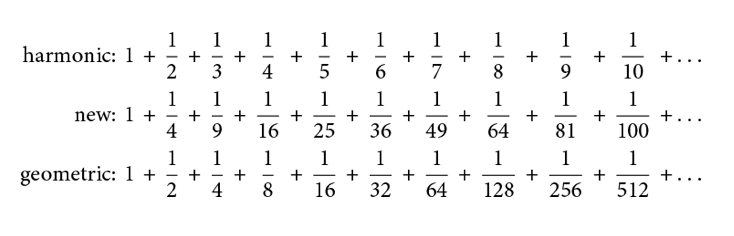
\includegraphics [scale=0.5] {new_series.png} \end{center}

The trick is to find another series which we can show converges (it's not one I've seen before).  

Alcock gives the formula for the sum, and we need to prove this by induction.  Leaving off the first term

\[ \frac{1}{1 \cdot 2} + \frac{1}{2 \cdot 3} + \frac{1}{3 \cdot 4} + \dots + \frac{1}{n(n+1)} = 1 - \frac{1}{n+1} \]
As $n \rightarrow \infty$, this is equal to $1$.

Before we get started, it is fair to ask where this formula comes from.  On the one hand, we note that 
\[ \frac{1}{n(n+1)} > \frac{1}{(n+1)^2} \]
so it will clearly do the job for us, term by term.  Alternatively, we could write
\[ \frac{1}{n(n-1)} > \frac{1}{n^2} \]
We may have to drop a term or two at the very beginning to line things up, but this is never a problem.

Now, we notice that
\[ \frac{1}{n(n+1)} = \frac{1}{n} - \frac{1}{n + 1} \]
In other words, any sum will be a telescoping sum.  So the result is simple, just what we had above with a different symbol.

\[ \sum_{n=1}^{n=k} \frac{1}{n} - \frac{1}{n + 1} = 1 - \frac{1}{k + 1} \]

Now for the proof by induction.  Clearly this works for the base case.  We need to add the next term (for $n+1$) from the left-hand side to the right-hand side and show that it reduces to the correct form.

\[ (1 - \frac{1}{n+1}) + \frac{1}{(n+1)(n+2)} \]
\[ = 1 - \ [ \ \frac{1}{n+1} - \frac{1}{(n+1)(n+2)} \ ]  \]
\[ = 1 - \ [ \ \frac{n + 2 - 1}{(n+1)(n+2)} \ ]  \]
\[ = 1 - \ [ \ \frac{1}{n+2} \ ]  \]
which is indeed the sum on the right updated from $n$ to $n+1$.  So the solution is correct, the answer is finite, and thus the series does converge.

Then, comparison with our series shows the one which we just proved convergent, is bigger term by term.  So our series converges as well.

\[ \frac{1}{1 \cdot 2} + \frac{1}{2 \cdot 3} + \frac{1}{3 \cdot 4} + \frac{1}{4 \cdot 5}  + \dots \]
\[ \frac{1}{2 \cdot 2} + \frac{1}{3 \cdot 3} + \frac{1}{4 \cdot 4} + \frac{1}{5 \cdot 5}  + \dots \]

The second series is clearly smaller than the first, which is equal to $1$.

This is a bit of a sneaky example, because the sum (including the first term) is a famous series related to $\pi$, found in the reference at the end of the last section:

\[ \frac{\pi^2}{6} = \sum_1^{\infty} \frac{1}{k^2} \]

\subsection*{The fly and the train}

Two trains (or bicycles) are 20 miles apart and headed directly toward each other at a speed of 10 mph. A fly starts from the front of the train on the left, flies at a speed of 15 mph to the tip of the train on the right, then turns around immediately and flies back to the first. This cycle continues until the trains meet, ending everything.

How far does the fly fly?

\url{http://mathworld.wolfram.com/TwoTrainsPuzzle.html}

There is a hard way and an easy way to do this problem.  The story was that being shown the problem, Johnny Von Neumann did it instantly, and when asked how he did it, said that he used infinite series (this is the hard way). 

We will sum an infinite series.  It takes a little time to set up, but we know how to solve it.  Let's do one round to see what happens.
 
$\circ $  initial distance between trains:  $20$ miles

$\circ $  relative speed of fly to second train:  $25$ miles per hour

$\circ $  time to meet:  $20/25 = 0.8$ hour

$\circ $  distance the fly travels:  $0.8 \times 15 = 12$ miles

$\circ $  each train travels $0.8 \times 10 = 8$ miles

$\circ $  distance separating the trains after this round:  $4$ miles

The ratio $4/20 = 1/5$ miles allows us to set up the series:

\[ 12 + 12 \frac{1}{5} + 12 (\frac{1}{5})^2 + \dots \]
\[ 12 \ [ \ 1 + \frac{1}{5} +  (\frac{1}{5})^2 + \dots \ ] \]
\[ 1/1-r = 5/4 \]
Total distance = $15$ miles.

The easy way is that the closing speed of the two trains, $20$ miles per hour, is the same as the initial separation of $20$ miles, so the trains meet in 1 hour.  The fly travels $15$ miles in one hour.

We should be able to get the series from the train speeds, the fly speed and the initial distance.  Let
\[ d =  \text{ initial distance/(train speed + fly speed)} = \frac{20}{15 + 10} \]

The common ratio is
\[ r = 1 - d = \frac{1}{5} \]

The initial value $a$ is the fly speed times $d$.

Here is a nice graphic for a variant that I found on the web.

\begin{center} 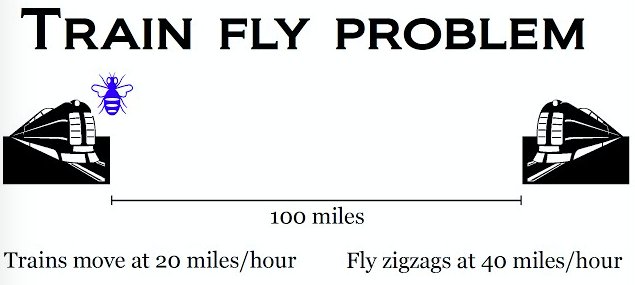
\includegraphics [scale=0.6] {fly_train.png} \end{center}

\end{document}